\documentclass[12pt, a4paper]{report}
\usepackage[utf8]{inputenc}
\usepackage{fourier} %for the font
\usepackage[english,french]{babel} %To use the csquotes package without warnings
\usepackage[autostyle]{csquotes} %for the quotes -> \enquote{the quote}
\usepackage{wrapfig} % For using images wrapped inside some text
\usepackage{graphicx}   % For images 
\usepackage{subcaption} % for multiple image captions
\usepackage{array}      %for tables
\usepackage[final]{pdfpages} % To Include PDFs

\newcolumntype{P}[1]{>{\centering\arraybackslash}p{#1}}
\title{Medical Structure Visualization}
\author{Malek Benzerga}

\usepackage{hyperref} %for a clickable titles
\hypersetup{  %for a clickable titles suite
    colorlinks,
    citecolor=black,
    filecolor=black,
    linkcolor=black,
    urlcolor=black
}


\usepackage[font=small,labelfont=bf]{caption}
\def\figurename{\textbf{Figure }}

\hypersetup{
pdftitle={VISUALIZATION OF HEALTH DATA IN A MEDICAL SECTOR},
pdfsubject={Master Graduation Project},
pdfauthor={Benzerga Malek kheira},
pdfkeywords={Visualization; Medical data; Graphical Representation; Modeling; XML; Personalized DashboardL}
}


%		Header		%		
\usepackage{fancyhdr}
\pagestyle{fancy}
\rhead{\thepage}
\lhead{\leftmark}

%%%%%%%%%%%%%%%%%%%%
\providecommand{\keywords}[1]{\textbf{\textit{Mots clés---}} #1}
\providecommand{\keywordz}[1]{\textbf{\textit{Keywords---}} #1}

\providecommand{\keywordEN}[1]{\textbf{\textit{Keywords---}} #1}

\providecommand{\keywordFR}[1]{\textbf{\textit{Mots clés---}} #1}
%%%%%%%%%%%%%%%%%%%%%%%
\setcounter{tocdepth}{4}
\setcounter{secnumdepth}{4}
\newcommand{\comment}[1]{}

\usepackage{csquotes} % for the quotes

\begin{document}
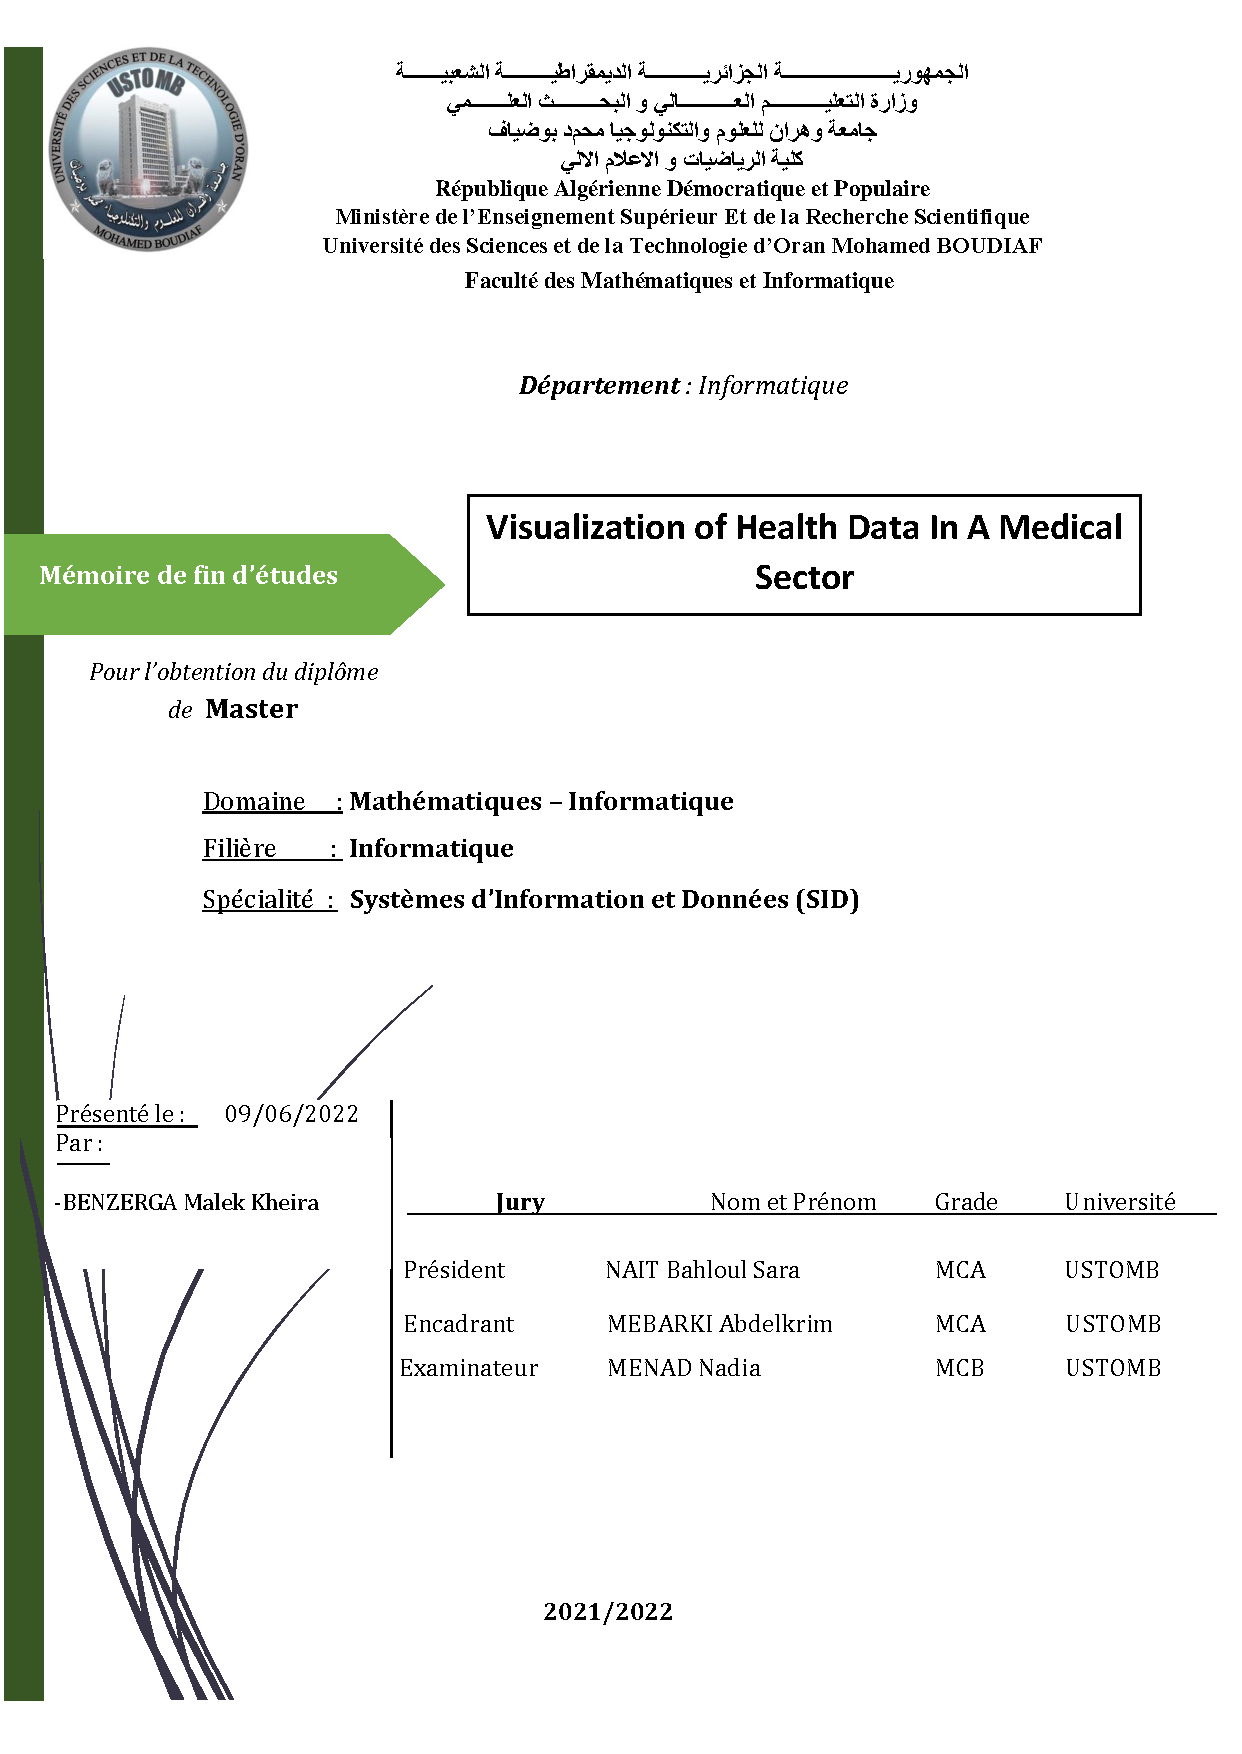
\includepdf[pages=-]{parts/pagedegarde.pdf}
\begin{titlepage}
    \begin{center}
        MASTER DEGREE OF DATA \& INFORMATION SYSTEMS
        \vspace*{1cm}
        \\Department of Computer Science\\
        University of Science and Technology of Oran - Mohamed Boudiaf\\
        Oran, Algeria\\
 
        {\large
        \textbf{Visualisation of health data in a medical sector}}
 
        \vspace{1cm}
         Authored by
             
        \vspace{0.5cm}
 
        \textbf{Malek kheira Benzerga}


        \vspace{0.5cm}
         Supervised by
             
        \vspace{0.5cm}
 
        \textbf{Abdelkarim Mebarki}
 
        \vfill
             
        
        \vspace{0.8cm}
      
        
\includegraphics[width=0.3\textwidth]{images/others/usto.jpg}
             
        \vspace{0.5cm}
        Department of Computer Science\\
        University of Science and Technology of Oran - Mohamed Boudiaf\\
        Oran, Algeria\\
        2022
             
    \end{center}
 \end{titlepage}
\newenvironment{acknowledgement}{
  \vspace*{\fill}
  \begin{center}%
    \bfseries Acknowledgements \& Dedication
  \end{center}}%
  {\vfill}
  
  \thispagestyle{empty}
  
\begin{acknowledgement}

    I want to present all my gratitude to my supervisor Mr MEBARKI Abdelkarim who was always there to answer my questions, provide his insights, and to  guide me in the right direction when it was needed and for accepting to supervise and helping me. 
    
    I present a special thanks to all the examiners Miss NAIT Bahloul and Miss MENAD Nadia for accepting to review and judge my thesis.
 
    I would also like to take this opportunity to thank all the friends who have always been there for me: Oussama, Meriem, Houari, Soumia, Sirine, and to my colleagues from the UDev scientific club.
 
    Finally, I wish to express my very profound gratitude to my family and special thanks to my parents for providing me with unconditional support and continuous encouragement throughout my years of study. This accomplishment would not have been possible without you. Thank you!



\begin{flushright}
\textbf{Malek.}
\end{flushright}
\end{acknowledgement}

\clearpage
\begin{selectlanguage}{english}
    
    \begin{abstract}
        
        The care of patients in a medical structure is provided by medical and paramedical staff. Coordination between staff involved in healthcare requires efficient and synchronized communication. The presence of visual representations in this communication adds a dimension to the data which can improve their reading, their interpretations, and thus accelerate the response time. 
        \bigbreak
        In this project, four major points will be addressed: healthcare and its data, information visualization  in this field, the different data management systems for multiple medical actors and the visualization system proposed to display personalized dashboards for different actors.
 \newline 

        \begin{keywordEN}
            Visualization; Medical data; Graphical Representation; Modeling; XML; Personalized Dashboard.\\
            
        \end{keywordEN}
        
    \end{abstract}
\end{selectlanguage}


\begin{selectlanguage}{french}
    
    \begin{abstract}
        
        La prise en charge des patients dans une structure médicale est assurée par du personnel médical et paramédical. La coordination entre le personnel impliqué dans les soins nécessite une communication efficace et synchronisée. La présence de représentations visuelles dans cette communication ajoute une dimension aux données qui peut améliorer la lecture de ces données, leurs interprétations, et ainsi accélérer le temps de réponse. 
        \bigbreak
 
        Dans ce projet, quatre points majeurs seront abordés : la santé et les données, la visualisation de l'information dans ce domaine, les différents systèmes de gestion de données pour de multiples acteurs médicaux et le système de visualisation proposé pour afficher des tableaux de bord personnalisés pour différents acteurs.
        \newline 

        \begin{keywords}
            Visualisation; Données médicales ; Représentation graphique; La modélisation; XML; Tableau de bord personnalisé.\\
            
        \end{keywords}
        
    \end{abstract}
\end{selectlanguage}

\tableofcontents
\listoffigures
\listoftables 
 

\chapter{Introduction}

Health has played an important role in human history, helping civilization, behind the curtains, to evolve into the society of today\cite{xu2020privacy}. Recently, the healthcare sector has witnessed the development of a wide range of IoT devices and applications\cite{nasiri2019security}. And a new field has been unlocked: Healthcare information technology (HIT).

\section{Background}
Healthcare information technology (HIT) has been defined as \enquote{the application of information processing involving both computer hardware and software that deals with the storage, retrieval, sharing, and use of healthcare information, data, and knowledge for communication and decision making\cite{brailer2004decade}} where the oil of it is the Medical Informatics as Morris F Collen defines it: \enquote{Medical informatics is the application of computer technology to all fields of medicine-medical care, medical teaching and medical research}; in other words The medical informatics is the foundation for understanding and practice of the up-to-day medicine. Its basic tool is the computer, the subject of studying and the means by which the aspects and achievement in the new knowledge in studying of a man, his health and disease and functioning of the total health activities is performed\cite{masic2013history}.

Medical informatics as a discipline is still young, in particular when you compare it with other medical disciplines. However, within the past decades, societies in general, and medicine and healthcare in particular, have tremendously changed by the adoption of health information technology. This change has significantly impacted the healthcare field as well\cite{haux2010medical}. As a result,  health information technology improves patient’s safety by reducing medication errors, reducing adverse drug reactions, and improving compliance to practice guidelines. There should be no doubt that health information technology is an important tool for improving healthcare quality and safety\cite{alotaibi2017impact}.


\section{Problem \& motivation}
With the progress of health information technology the healthcare data is increasingly digitized and, like in most other industries, data is growing in Velocity, Volume and Value. According to Statista\cite{HealthcareDataVolume}, the amount of global healthcare data is expected to increase dramatically by the year 2020. Early estimates from 2013 suggest that there were about 153 exabytes of healthcare data generated in that year. However, projections indicate that there could be as much as 2,314 exabytes of new data generated in 2020 (Figure \ref{fig:dataGenerated}).

\begin{figure}[h!]
    \center
    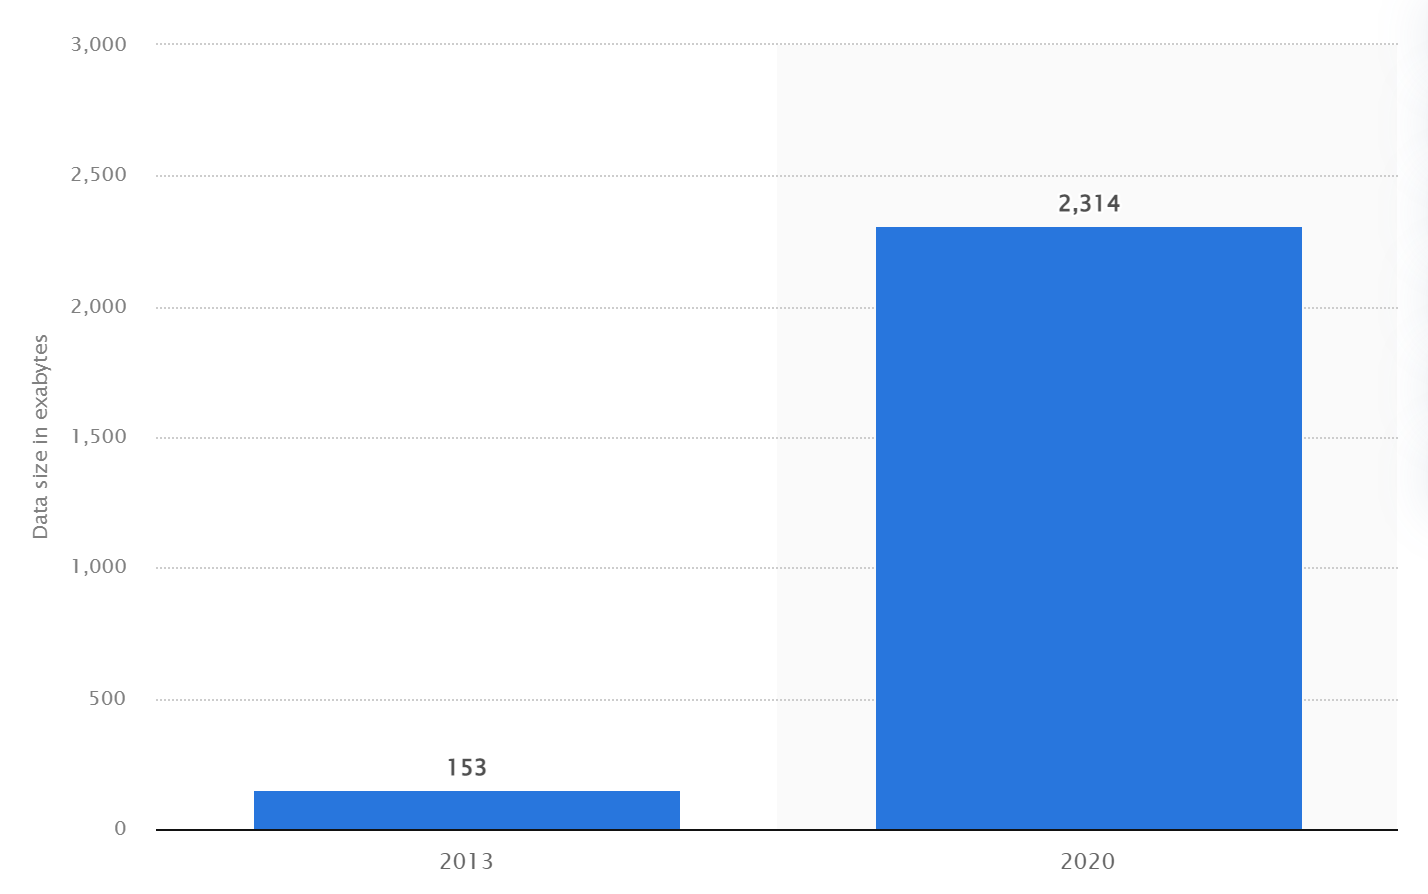
\includegraphics[width=0.75\textwidth]{images/intro/sista.PNG}
    \caption{Total amount of global healthcare data generated in 2013 and a projection for 2020* (in exabytes).}
    \label{fig:dataGenerated}
  \end{figure}

Health Data Management is the practice of making sense of this data and managing it to the benefit of healthcare organizations, practitioners, and ultimately patient well being and health, It enables the integration and analysis of medical data to make patient care more efficient, and extract insights that can improve medical outcomes, while protecting the security and privacy of the data. In the past forty years, medical data began a transition from purely paper-based tracking to digitized information. Even today, many types of medical data have yet to be digitized, or have not yet been integrated into Health Data Management systems. Some of the important challenges facing health data professionals today are\cite{HealthDataManagement}:
\begin{itemize}
    \item \textbf{\textit{Fragmented data:}} medical data can be structured data in spreadsheets or databases, images or video files, digital documents, scanned paper documents, or may be stored in specialized formats such as the DICOM format used for MRI scans. Data is widely duplicated, collected multiple times and stored in different versions by healthcare providers, public health organizations, insurance bodies, pharmacies, and patients themselves. There is no one source of truth for information on patient well being.
    \item \textbf{\textit{Changes to data:}} medical data constantly changes as do the names, professions, locations and conditions of patients and physicians. Patients undergo numerous tests and are administered many types of treatment over the years, and the treatments and medications themselves evolve over time. New types of medical treatment, such as telehealth models, create new types of data.
    \item \textbf{\textit{Regulations and compliance:}} medical data is sensitive and must adhere to government regulations, such as the USA Health Insurance Portability and Accountability Act (HIPAA). Data discovery challenges and poor data quality make it much more difficult to perform the required audits and meet regulatory requirements and limits the diversity of data healthcare providers can use for the benefit of patients.
  \end{itemize}




\section{Purpose \& delimitations}

The goal of this work is to design a visualization system for medical data in a conventional common language between the different health actors.
 
We intend to achieve our goal by designing a warehouse system that brings  data from different sources together, and structures it using the eXtensible Markup Language (XML).
 \newline
 \textbf{First}, we created a data warehouse that takes care of the data integration.\newline 
 \textbf{Second}, we integrated the focus data in a structured form using XML.\newline
 \textbf{Third}, we designed a visual presentation after the data processing and formatting.

\section{Document structure}
This document is presented in 6 chapters, starting with the chapter1: Introduction, in which we present a bit of background of the topic and then delve into formally defining the problem we intend to tackle, followed by a brief description of what lies within and beyond the scope of this work.
 
In Chapter 2: Health sector \& Data, we present the healthcare environment including the principal actors, activities, and the type of data generated from each one. Then we presented the Medical records management and its various electronic types and how important security is to them.
 
In chapter 3: Information Visualization, we present its definition, then we explain the visualization pipeline: how it deals with data, then we move to the data warehouse and its data integration approaches.
 
 Next comes chapter 4: Contribution \& Discussion, we talk about the work objectives then we go through several related work reviews and then present the proposed work. Chapter 5: Implementation, a chapter about the implementation of the system, which tools are introduced and results are displayed using screenshots and diagrams.
 
Finally, in chapter 5: Conclusion \& Future work, the results and insights gained through the journey of making the proposed solution, few conclusions drawn and perspectives on what could be enhanced moving forward with this project.

\chapter{Health sector \& Data}

Healthcare is a multi-dimensional system established with the sole aim for the prevention, diagnosis, and treatment of health-related issues or impairments in humans. There is three components of a healthcare system\cite{dash2019big}:
\begin{itemize}
    \item The health professionals (physicians or nurses): belong to various health sectors like dentistry, medicine, midwifery, nursing, psychology, physiotherapy, and many others.
    \item Health facilities (clinics, hospitals for delivering medicines and other diagnosis or treatment technologies).
    \item Financing institution supporting the former two.
  \end{itemize}
  Healthcare is required at several levels depending on the urgency of situation:
  \begin{enumerate}
    \item \textbf{\textit{Primary care:}} Professionals serve it as the first point of consultation.
    \item \textbf{\textit{Secondary care:}} acute care requiring skilled professionals.
    \item \textbf{\textit{Tertiary care:}} advanced medical investigation and treatment.
    \item \textbf{\textit{Quaternary care:}} highly uncommon diagnostic or surgical procedures.
  \end{enumerate}
 At all these levels, the health professionals are responsible for different kind of information such as a patient's medical history (diagnosis and prescriptions related data), medical and clinical data (like data from imaging and laboratory examinations), and other private or personal medical data


Regardless of what form it takes, data has the potential to tell stories, identify cost savings and efficiencies, new connections and opportunities, and enable improved understanding of the past to shape a better future\cite{Zillner2016}.

The term “big data” has become a buzzword in recent years, with its usage frequency having doubled each year in the last few years according to common search engines (Figure \ref{fig:bigDataGoogleScholar}).

\begin{figure}[h!]
    \center
    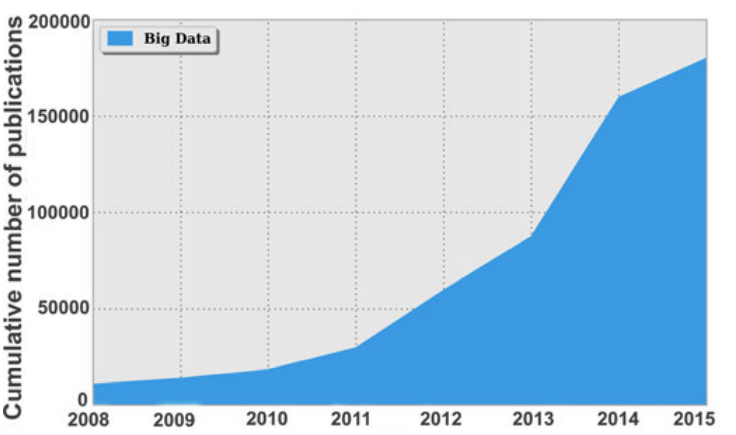
\includegraphics[width=0.75\textwidth]{images/chapter1/publication_big_data.PNG}
    \caption{Cumulative number of publications referring to “big data” indexed by Google Scholar.}
    \label{fig:bigDataGoogleScholar}
  \end{figure}
 
Big data is a vague term with a definition that is not universally agreed upon. A definition by Demchenko et al\cite{demchenko2012addressing} who define Big Data by five V’s: Volume, Velocity, Variety, Veracity, and Value. Volume pertains to vast amounts of data, Velocity applies to the high pace at which new data is generated, Variety pertains to the level of complexity of the data, Veracity measures the genuineness of data, and Value evaluates how good the quality of the data is in reference to the intended results.


If we trace the relationship between the use of the term big data per health research , we can easily infer the growth of medical informatics (Figure \ref{fig:bigDataHealthResearch}). Big data in health is concerned with meaningful datasets that are too big, too fast, and too complex for healthcare providers to process and interpret with existing tools\cite{andreu2015big}.
\begin{figure}[h!]
    \center
    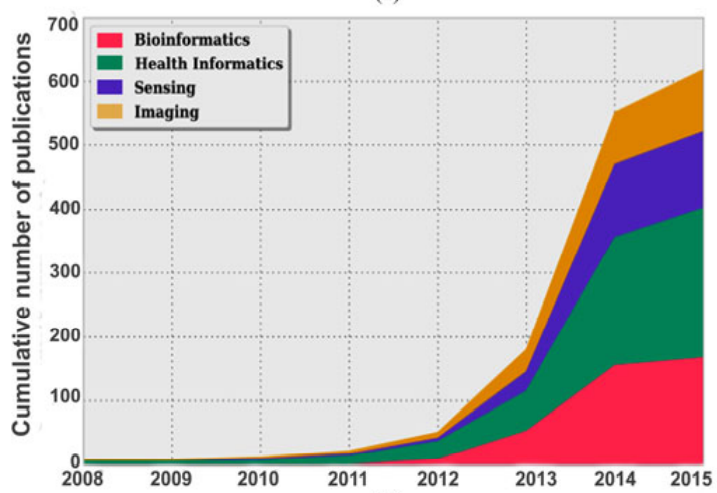
\includegraphics[width=0.75\textwidth]{images/chapter1/health_publication_bigData.PNG}
    \caption{Cumulative number of publications per health research
    area referring to “big data,” as indexed in IEEE Xplore, ACM Digital library, PubMed (National Library of Medicine, Bethesda, MD), Web of Science, and Scopus.}
    \label{fig:bigDataHealthResearch}
  \end{figure}

  \newpage
There are numerous current areas of research within the field of Health Informatics, including Bioinformatics, Image Informatics (e.g. Neuroinformatic), Clinical Informatics, Public Health Informatics, and also Translational BioInformatics (TBI). Research done in Health Informatics (as in all its subfields) can range from data acquisition, retrieval, storage, analytics employing data mining techniques, and so on.
\bigbreak
Data gathered for Health Informatics research does exhibit many of these qualities. Big Volume comes from large amounts of records stored for patients: for example, in some datasets each instance is quite large (e.g. datasets using MRI images or gene microarrays for each patient), while others have a large pool with which to gather data (such as social media data gathered from a population). Big Velocity occurs when new data is coming in at high speeds, which can be seen when trying to monitor real-time events whether that be monitoring a patient’s current condition through medical sensors or attempting to track an epidemic through multitudes of incoming web posts (such as from Twitter). Big Variety pertains to datasets with a large amount of varying types of independent attributes, datasets that are gathered from many sources (e.g. search query data comes from many different age groups that use a search engine), or any dataset that is complex and thus needs to be seen at many levels of data throughout Health Informatics.

\newpage
Schematically, several health-related activities can be distinguished\cite{martigneneVisualisationUnifieeDonnees}:
\begin{itemize}
  \item Pre-admission, admission and administrative discharge activities.
  \item T2A invoicing or valuation activities.
  \item Care activities in the accommodation service.
  \item Activities in operating theaters and technical platforms.
  \item Laboratory activities.
  \item Imaging activities.
\end{itemize}

For each activity, different types of data are generated. In France and most developed countries, the following data is collected and digitally available (in chronological order)\cite{ATIHAgenceTechnique,boracle2009detection}:
\label{chap:healthData}
\begin{enumerate}
  \item \textbf{Administrative data} related to patient movements (identity, dates, places, etc.), demographic (age, sex, place of residence, etc.) and insurance (health coverage, etc.).
  \item \textbf{Results of biological analyses}, generally taken by nurses and analyzed by professionals or by robots.
  \item \textbf{Medical data} produced automatically by autonomous medical devices. These devices can be implantable or external.
  \item \textbf{Data relating to the drugs administered to the patient},
  generally by nurses or doctors, possibly as part of a diagnostic or therapeutic procedure.
  \item \textbf{Data relating to medical devices} implanted in the patient during surgery.
  \item \textbf{Data relating to medical procedures}, whether diagnostic or therapeutic. These data are generally coded by the producer, sometimes by the machine which produces them.
  \item \textbf{Comments} in free text, possibly formalized in letters or reports.
  \item \textbf{Medical diagnoses}, coded a posteriori by the doctors who treated the patient, or by specialized technicians reading the letters\cite{emmanuelchazardReutilisationFouilleDonnees2017}.
\end{enumerate}


\newpage

This data can be structured (which can be used directly by an algorithm) or unstructured (they are stored without a predefined format, such as the text of reports or medical letters, and are interpreted by humans). Machines generally produce raw structured information (eg medical biology measurements), while healthcare professionals exchange unstructured information with high interpretative value (eg a diagnosis). 
Medical records are created by aggregating information from different sources: (Table \ref{tab:sourceTable}) gives an overview of this data\cite{martigneneVisualisationUnifieeDonnees}. 


\begin{table}[h!]
    \centering
    \begin{tabular}{|m{0.45\linewidth}|m{0.20\linewidth}|m{0.35\linewidth}|}
        \hline
        Category                                         & Nature                                                        & Structure                                                   \\
        \hline
        \textbf{Administrative data}                                           & Values, Text                                 & Structured                                       \\
        \hline
        \textbf{Communications between caregivers} (Transmissions and medical observations, medical letters, reports)                      & Text              & Unstructured                                               \\
        \hline
        \textbf{Data managed by centralized pharmacies}                       & Values         & Structured                    \\
        \hline
        \textbf{Medical biology results}                               & Values, Text & Structured                           \\
        \hline
        \textbf{Data from monitoring devices}     & Values                                                         & Structured                                                      \\
        \hline
        \textbf{Image Data Images}                             & Images, Text                                                & Unstructured                               \\
        \hline
        \textbf{PMSI data and codes}  & Codes, Values                                                        & Structured                                              \\
                               
        \hline
    \end{tabular} 

    \caption{Origin, nature and structure of medical record data.}
    \label{tab:sourceTable}
\end{table}


\section{Medical records management}
Self-tracking and documenting information about aspects of one’s personal and daily life has a long history. It is an effective method which helps us to learn more about ourselves, rather than depending on our limited memory\cite{alrehielyEvaluatingDifferentVisualization}.


The medical record is a multifunctional document that is used to communicate and document critical information about patients’ medical care among health care professionals. Comprehensive medical records are a cornerstone in the quality and efficiency of patient care during the hospitalization and in subsequent follow-up visits, as they can provide a complete and accurate chronology of treatments, patient results and future plans for care\cite{wong2009developing}, it involves many kinds of records, including patient charts, x-rays, images, scans, and even emails. Additionally, it involves making sure all of these items are accessible, safe, and secure.
There are multiple electronic records used in the healthcare.
\subsection{Electronic medical record}
Electronic medical record (EMR) systems, defined as "an electronic record of health-related information on an individual that can be created, gathered, managed, and consulted by authorized clinicians and staff within one health care organization,"  have the potential to provide substantial benefits to physicians, clinic practices, and health care organizations. 

It  is a digital version of the paper medical record that has been used for years and it will contain the patient’s medical and surgical history, allergy information, treatment history, current, and past prescriptions, and other pertinent information that can be used in making future medical decisions\cite{WheelWhatAre}. These systems can facilitate workflow and improve the quality of patient care and patient safety\cite{ElectronicMedicalRecord}.

\subsection{Electronic health record}
An Electronic Health Record (EHR) is an electronic version of a patient's medical history, that is maintained by the provider over time, and may include all of the key administrative clinical data relevant to that persons care under a particular provider, including demographics, progress notes, problems, medications, vital signs, past medical history, immunizations, laboratory data and radiology reports. The EHR automates access to information and has the potential to streamline the clinician's workflow.  It also has the ability to support other care-related activities directly or indirectly through various interfaces, including evidence-based decision support, quality management, and outcomes reporting. 
 
EHRs are the next step in the continued progress of healthcare that can strengthen the relationship between patients and clinicians.  The data, and the timeliness and availability of it, will enable providers to make better decisions and provide better care\cite{ElectronicHealthRecords}.


\subsection{The Difference Between EMR \& EHR}
Both the EMR and EHR contain electronic versions of a patient's medical history. Most of the information in an EMR goes into an EHR.


The EMR can contain medical history, diagnoses, medications, immunizations and dates, allergies, etc. Often, a patient needs to ask for a printed copy of an EMR to share with another medical provider.


The EHR contains similar details as the EMR, but also other relevant data like information from wearable devices, demographics, and insurance information. It can also contain lab data and imaging reports that come from other offices or practices. Assuming the software is compatible, other offices and practices can access the information within an EHR to help coordinate care and make clinical decisions\cite{KeyMaintainingMedical} (Table \ref{tab:EMRvsEHR}) gives an overview of this difference:
\begin{table}[h!]
    \centering
    \begin{tabular}{|m{0.50\linewidth}|m{0.50\linewidth}|}
        \hline
        \textbf{EMR (electronic medical record)}                             & \textbf{EHR (electronic health record)}                                  \\
        
        \hline
        Medical and clinical data gathered in one provider's office         & Medical and clinical data gathered from many providers' offices and hospitals     \\
        
        \hline
        Narrower view                       & Broader view        \\
        
        \hline
        Digital version of a paper chart in one office                       & Digital version of varied health information        \\
        
        \hline
        Not designed for sharing                             & Designed for sharing outside of an individual medical practice       \\
        
        \hline
        Providers use mainly for diagnosis and treatment     & Providers have access to many diagnostic tools to make decisions       \\
        
        \hline
    \end{tabular} 

    \caption{EMR vs. EHR: Similarities and Differences.}
    \label{tab:EMRvsEHR}
\end{table}


\subsection{Personal health record}
Electronic Personal Health Records (ePHRs) are a representation of health records connected to the care of a patient and are managed by the patient\cite{demirisPatientcenteredApplicationsUse2008}, unlike EHRs, which are managed by health care providers. ePHRs allow healthcare consumers the luxury of deciding which health information to share with healthcare providers\cite{tangPersonalHealthRecords2006}. Ozok et al.\cite{PaperbasedComputerbasedRecords} defined ePHR systems as patient centric, multi-functional, health management systems developed for managing and storing lifelong personal health information for various purposes from chronic to critical, medical and preventive care\cite{alsahafiOverviewElectronicPersonal2018}.

The information in an EHR is keyed in by healthcare providers and is only accessible to healthcare providers. In addition, an EHR might only contain information from a single healthcare provider. On the other hand, an individual will retain control of their own ePHR, which might encompass health information from different sources, such as various healthcare providers, as well as from the patient, as integrated ePHRs have the capability to incorporate data from different sources. Thus, at any one time, there may be various EHRs for one person but only one ePHR\cite{alsahafiOverviewElectronicPersonal2018}.
\begin{figure}[h!]
  \center
  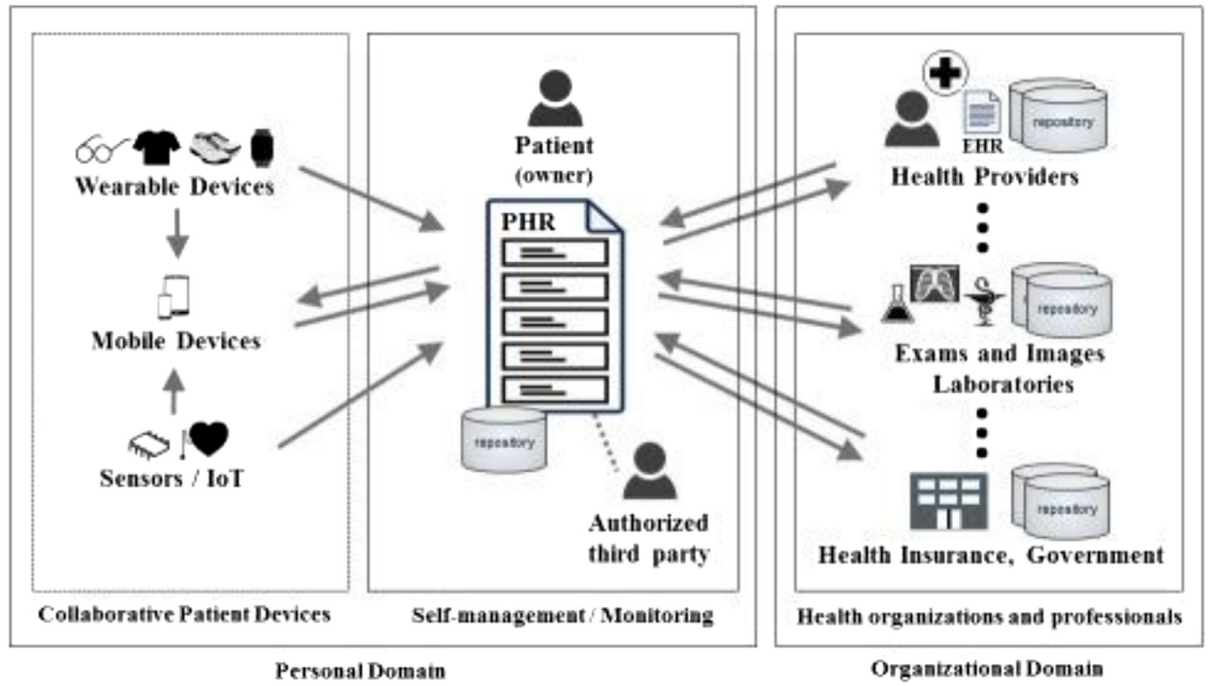
\includegraphics[width=0.75\textwidth]{images/chapter1/phr_ehr.PNG}
  \caption{Difference between an EHR and ePHR (Token from \cite{alsahafiOverviewElectronicPersonal2018}).}
  \label{fig:ehrvsphr}
\end{figure}

\section{Security in medical records management}
The actual technology of an electronic medical record seems to be falling into place. As the world moves more toward the use of telemedicine to preclude the movement of patients to more advanced facilities, the need for a fully functioning medical record is paramount.
One of the important ethical issues in electronic records management involves privacy. Privacy is the “claim of individuals to be left alone, free from surveillance or interference from other individuals, organizations, including state” (Laudon and Laudon 2005:159), privacy deals with the collection and use or misuse of data. Data is constantly being collected and stored on each of us. This data is often distributed over easily accessed networks and without our knowledge or consent\cite{ngoepeSecurityPrivacyEthics2011}.
 
 
There are a number of security dilemmas in electronic records management. There can be illegal access and use of records, data alteration and destruction (Stair and Reynolds 2006: 583).

\bigbreak
Typical cross-organisational e-health applications are\cite{ruotsalainenCrossplatformModelSecure2004}: 
\begin{itemize}
\item sharing of patient records among different healthcare professionals; 
\item access to distributed EHRs any place and any time; 
\item on-line teleconsultation, telemonitoring and assistance; 
\item patient—doctor consultation services;
\item patients’ access to their own EHRs.
\end{itemize}

\bigbreak
That is why Electronic health records management attracts significant international interest and sets the scenery for the establishment of a distributed, coalition-based, security policy enhanced records exchange framework among different medical domains. Several European projects have proposed candidate solutions for secure inter-operations between medical domains. In the HARP project, security profiles related to access rights are dynamically downloaded to the client side. The MEDITRAV EUproject attempts to overcome national or linguistic barriers by adopting the solution of a multilingual portable personal record. These approaches, pose mainly their research effort on the security requirements for effective electronic health record management, still they confront mainly to stable infrastructures\cite{belsisPervasiveSecureElectronic2005}.
\chapter{information visualization (infoVis)}

Human mind is very visual, following Williams et al., visualization is “a cognitive process performed by humans in forming a mental image of a domain space. In computer and information science it is, more specifically, the visual representation of a domain space using graphics, images, animated sequences, and sound augmentation to present the data, structure, and dynamic behavior of large, complex data sets that represent systems, events, processes, objects, and concepts”\cite{williamsVisualization1995}. The (Figure \ref{fig:roseDiagrame}) below presents the Florence Nightingale's 'Rose diagram' published in 1858 showing the reduction in the number of deaths in military hospitals in Scutari arising from the changes she instituted\cite{spence2001information} .

\begin{figure}[h!]
    \center
    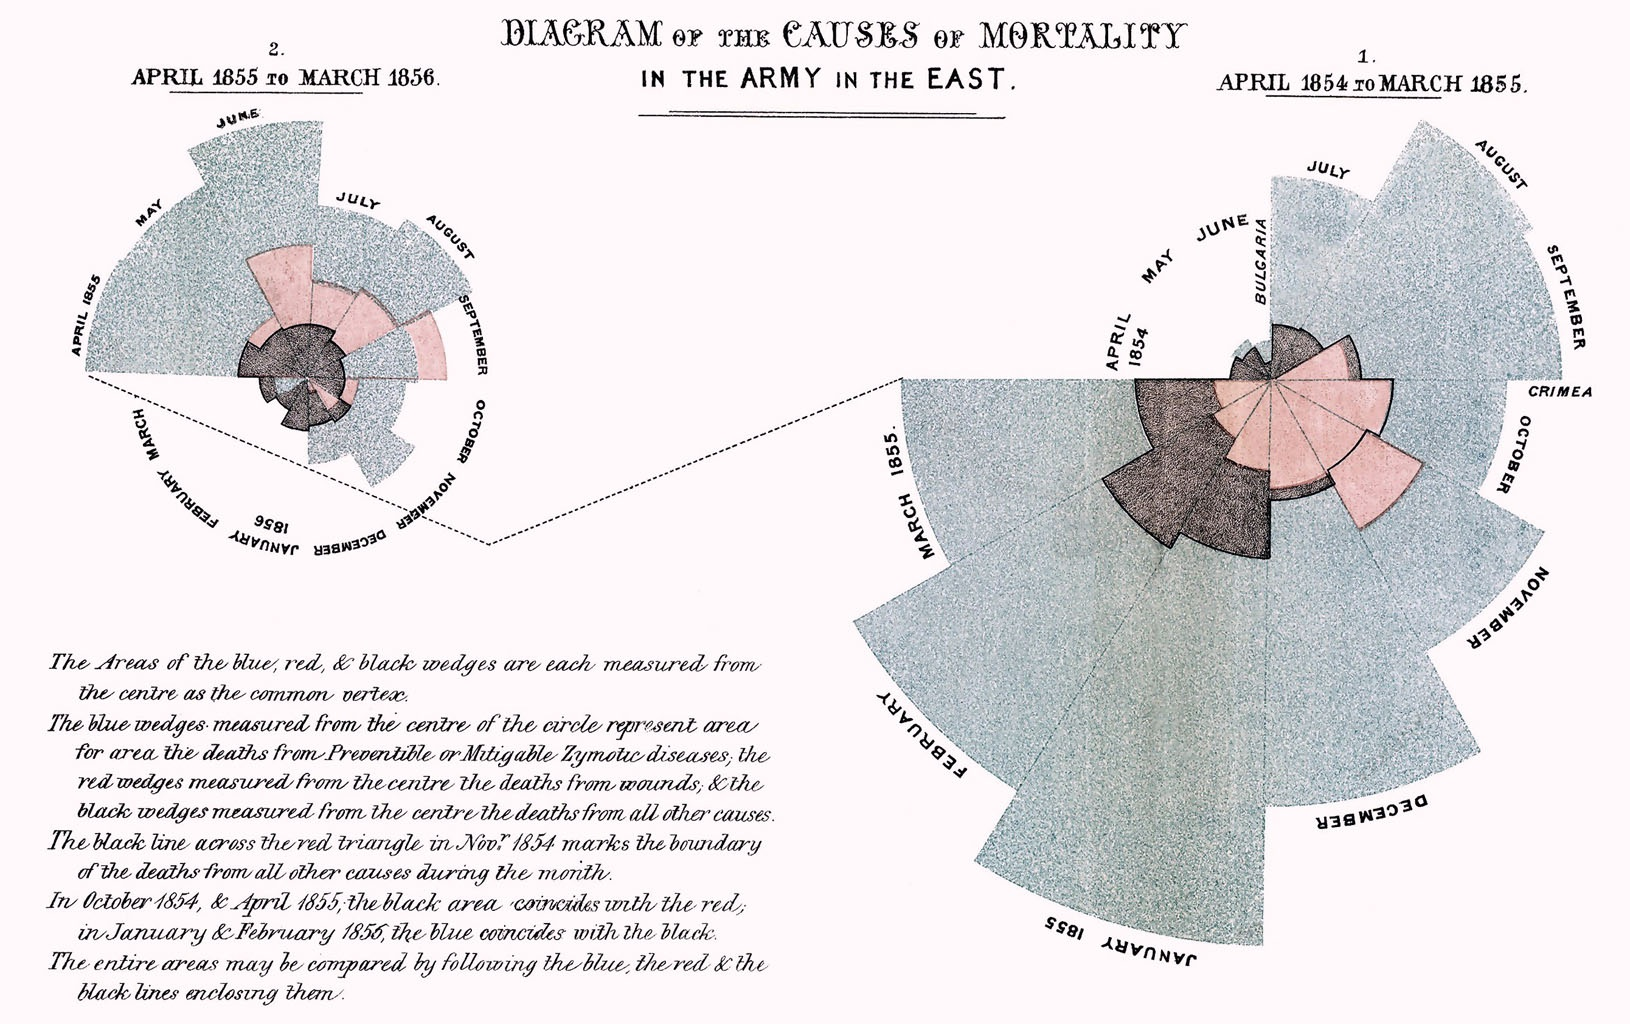
\includegraphics[width=0.78\textwidth]{images/chapter2/rose.jpg}
    \caption{Rose Diagrame}
    \label{fig:roseDiagrame}
  \end{figure}

 \newpage 
  Data visualization involves presenting data in graphical or pictorial form which makes the information easy to understand. It helps to explain facts and determine courses of action. It will benefit any field of study that requires innovative ways of presenting large, complex information\cite{spence2001information}.



  Traditionally, data visualization has been structured along two main fields: scientific visualization and information visualization. A third, newer field, called visual analytics has emerged in the past several years, as a bridge between and also an extension of the former two fields\cite{teleaDataVisualizationPrinciples2008}. In this paper we will focus mainly on the information visualization field.

\section{Difinition}
Information visualization (InfoVis) is the practice of representing data in a meaningful, visual way that users can interpret and easily comprehend, it is a research area that aims to aid users in exploring, understanding, and analyzing data through progressive, iterative visual exploration. With the boom in big data analytics, InfoVis is being widely used in a variety of data analysis applications in different domains, ranging from finance to sports to politics\cite{liuSurveyInformationVisualization2014}.
\bigbreak
Information visualizations are often created with an audience in mind and designed to display certain important information that they need to understand. With an idea of how the visualization will be used, using multiple tools (Column chart, Bar graph, Network graph, Stacked bar graph, Histogram, Line chart, Pie chart, Box plot, Bubble chart,  Dual-axis chart,…)\ref{fig:infoViseType} that can help users compare different values, show the bigger picture, track trends in the data, and understand different relationships between variables\cite{WhatInformationVisualization}. These tools follow the model of the visualization pipeline. 

\begin{figure}[h!]
  \center
  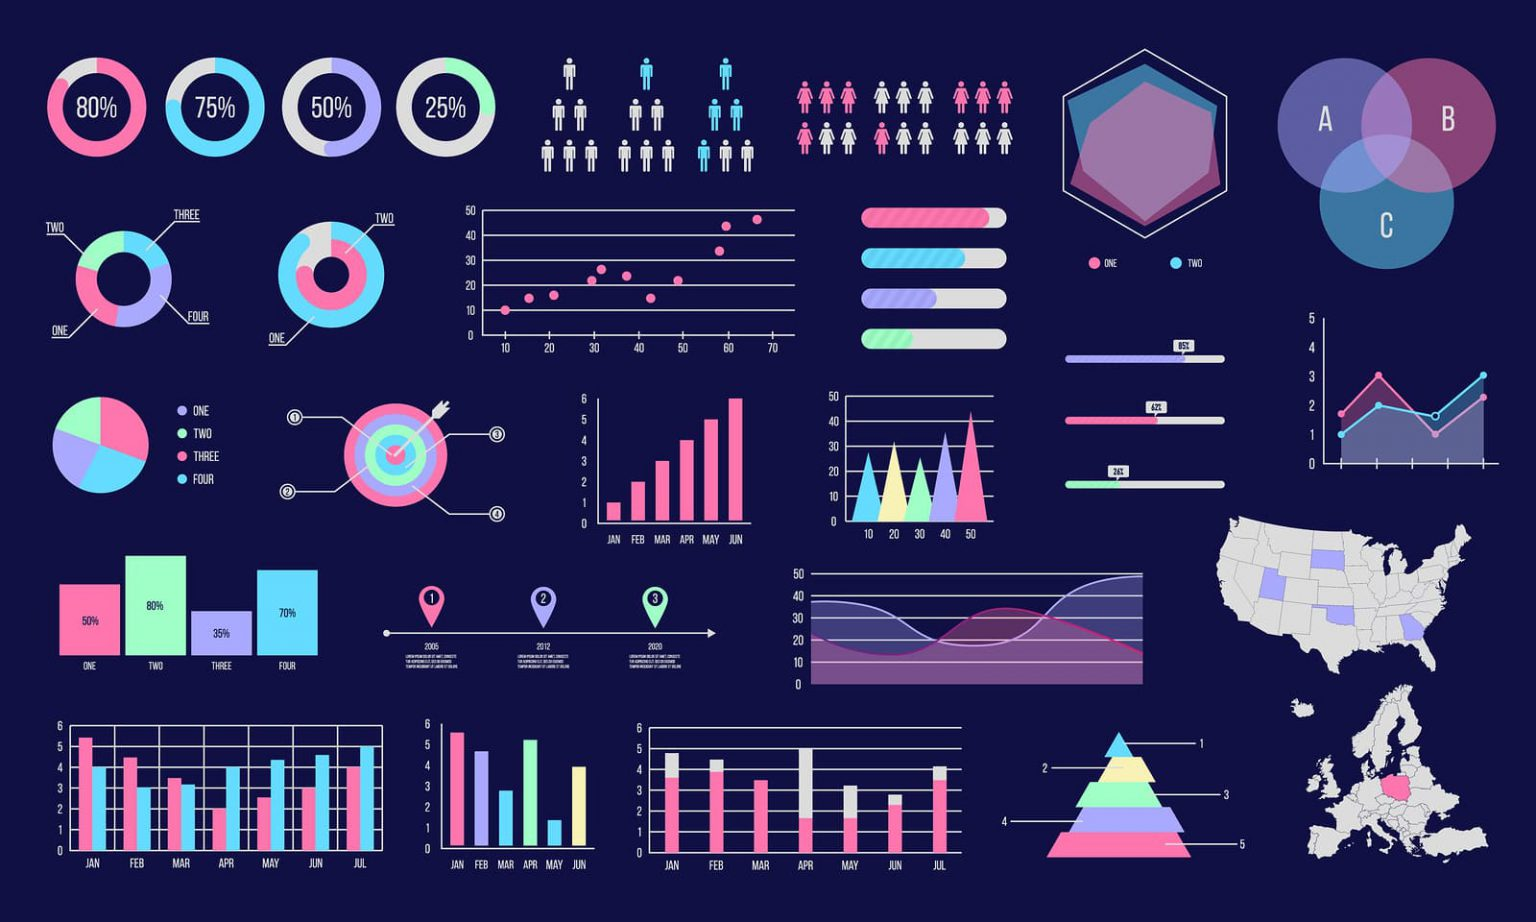
\includegraphics[width=0.60\textwidth]{images/chapter2/types-of-data-visualization.jpg}
  \caption{Information visualizations's tools}
  \label{fig:infoViseType}
\end{figure}

\section{Visualization pipeline}

A visualization pipeline embodies a dataflow network in which computation is described as a collection of executable modules that are connected in a directed graph representing how data moves between modules. In a \underline{basic} pipeline (Figure \ref{fig:simplepipeline}), there are three types of modules: sources, filters, and sinks. A source module produces data that it makes available through an output. File readers and synthetic data generators are typical source modules. A sink module accepts data through an input and performs an operation with no further result (as far as the pipeline is concerned). Typical sinks are file writers and rendering modules that provide images to a user interface. A filter module has at least one input from which it transforms data and provides results through at least one output\cite{morelandSurveyVisualizationPipelines2013}.

\begin{figure}[h!]
  \center
  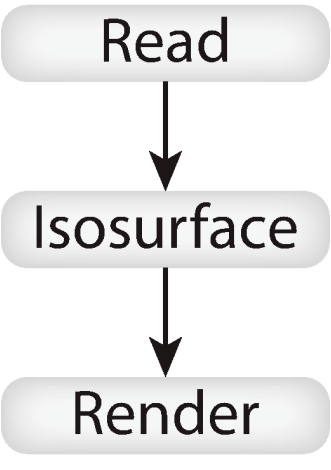
\includegraphics[width=0.20\textwidth]{images/chapter2/simplepipline.PNG}
  \caption{A simple visualization pipeline.}
  \label{fig:simplepipeline}
\end{figure}

\bigbreak
As science progresses, this model has been detailed, Figure \ref{fig:infovispipeline} provides an overview of the infoVis pipeline. It has five main modules: Data Analysis, Filtering, Mapping, Rendering, Image data, explained as follows:


\begin{figure}[h!]
  \center
  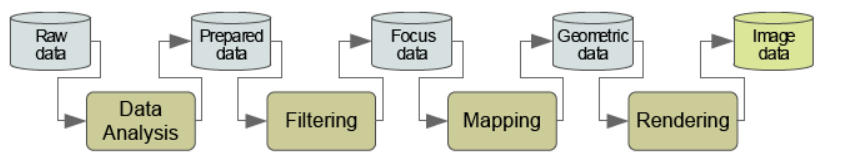
\includegraphics[width=0.75\textwidth]{images/chapter2/infoVispipeline.PNG}
  \caption{A simple visualization pipeline.}
  \label{fig:infovispipeline}
\end{figure}


 
\begin{enumerate}
  \item \textbf{\textit{Raw data:}} First, we have to import the data. This implies finding a representation of the original information we want to investigate in terms of a data set. Practically, importing data means choosing a specific dataset implementation and converting the original information to the representation implied by the chosen dataset in order to turn this data into information using Data analysis.
  \item \textbf{\textit{Data Analysis:}} Is the process of bringing order and structure to collected data. It turns data into information teams can use. Analysis is done using systematic methods to look for trends, groupings, or other relationships between different types of data\cite{DataAnalysisVisualization}, following this process:
  \begin{itemize}
  \item \textbf{\textit{Data Requirements Specification:}} The data required for analysis is based on a question or an experiment. Based on the requirements of those directing the analysis, the data necessary as inputs to the analysis is identified (e.g., Population of people). Specific variables regarding a population (e.g., Age and Income) may be specified and obtained. Data may be numerical or categorical\cite{DataAnalysisProcess}.
  \item \textbf{\textit{Data Collection:}} Guided by the requirements identified, Data can be collected through several sources, including online sources, computers, personnel, and sources from the community.
  \item \textbf{\textit{Data processing:}} The data that is collected must be processed or organized for analysis. For instance, these may involve placing data into rows and columns in a table format (known as structured data) for further analysis, often through the use of spreadsheet or statistical software\cite{DataAnalysisProcess}.
  \item \textbf{\textit{Data Cleaning:}} The processed and organized data may be incomplete, contain duplicates, or contain errors. Data Cleaning is the process of preventing and correcting these errors\cite{DataAnalysisProcess}.
  \item \textbf{\textit{Perform data analysis:}}  One of the last steps in the data analysis process is analyzing and manipulating the data. This can be done in a variety of ways depending on the cleaned data nature\cite{WhatDataAnalysis}.
  \end{itemize}
  The data analysis step produces the \underline{prepared data}.
  \item \textbf{\textit{Filtering:}} Data filtering is the process of choosing a smaller part of your data set and using that subset for viewing or analysis\cite{WhatDataFiltering}, this portion of data called \underline{focus data}. 
  \item \textbf{\textit{Mapping:}} Focus data are mapped to geometric primitives (e.g., points, lines) and their attributes (e.g., color, position, size); most critical step for achieving expressiveness and effectiveness.
  \item \textbf{\textit{Rendering:}} The rendering operation is the final step of the visualization process, rendering takes the geometric data created by the mapping operation and transforms it to an image data.
  \end{enumerate}
  







\section{TODO}
transition to the pipeline i will use.
re orgnizing l'enchainement d'idees + titles.
\section{Literature \& related works review}
talk about some related work.

\chapter{Technical background}
** i will talk about all the tech i used here 
\section{backend side}
different techs i used in the backend side (while manipulationg data and such)
\section{visualization side}
different techs i used in the visualization side (ploting and disign part)

\chapter{Implementation}
\section{Tools}
\section{Result}

\chapter{Conclusion and prespectives}
\chapter{Contribution \& Discussion}
\renewcommand{\thesection}{\arabic{section}}
		




\label{chapitre4}
		
		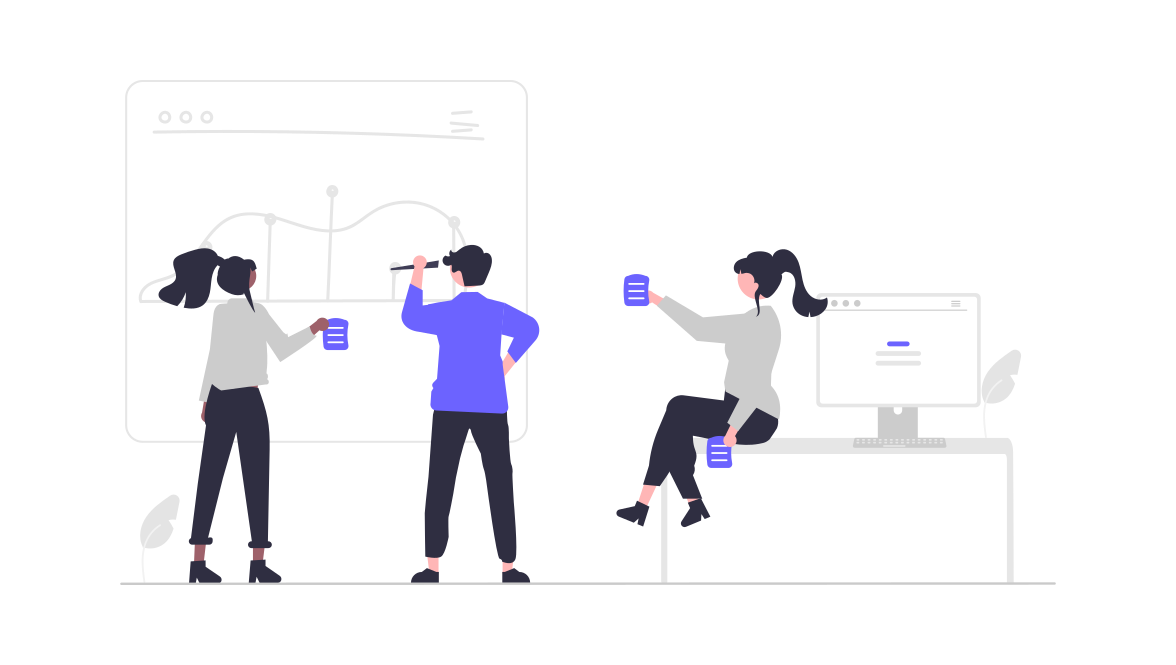
\includegraphics [width=1 \linewidth, height=0.8\textheight, keepaspectratio] {images/chaptersFigures/contribution.png}
		
	
		
    \newpage
    \thispagestyle{plain}

In this chapter we propose our data warehouse and visualization system for medical data that aims to manage the uncommon data from the various sources using a conventional common language between the different health actors.




\section{Work Objectives}
The aim of this work is to propose a data warehouse system that organizes data coming from different sources by producing a common language. We are interested in the step between Rendering and Data image in the pipeline process(\ref{fig:infovispipeline}). After reviewing and analyzing similar proposed works, we created our own visualization system for medical data in a conventional common language.





\section{Literature \& Related works review}
We present in this section architecture for healthcare data warehouses and solutions that attempt to integrate infoVis into medical data and medical structures which could be used by executive managers, doctors, physicians and other health professionals to support the healthcare process.  Medical data existing today in multiple sources with different formats makes it necessary to have certain data integration techniques. A healthcare data warehouse is therefore needed to integrate the different data sources into a central data repository and analyze this data.

\begin{itemize}
  \renewcommand{\labelitemi}{$\bullet$}
  \item \textbf{\textit{A Healthcare Data Warehouse for Cancer Diseases:}} Dr.Osama E.Sheta and Ahmed Nour Eldeen discussed in their paper\cite{shetaBuildingHealthCare2012} the implementation of a healthcare data warehouse for cancer diseases, they proposed  two stages approach for the building cancer data warehouse: 
  
  \begin{enumerate}
    \item \textit{Business Analysis:} Consist of business process analysis and business requirement analysis (Figure\ref{fig:cancerDiagrame}). \newpage
    \begin{figure}[h!]
      \center
      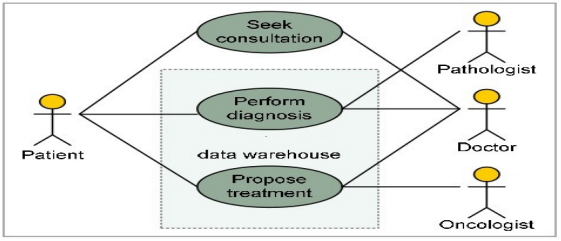
\includegraphics[width=0.75\textwidth]{images/chapter3/cancerDiagrame.PNG}
      \caption{Cancer data warehouse use case diagram.}
      \label{fig:cancerDiagrame}
    \end{figure}
    \item \textit{Architecture Design:} Data is imported from several sources and transformed within a staging area before it is integrated and stored in the production data warehouse for further analysis (Figure\ref{fig:cancersystem}).
     \begin{figure}[h!]
      \center
      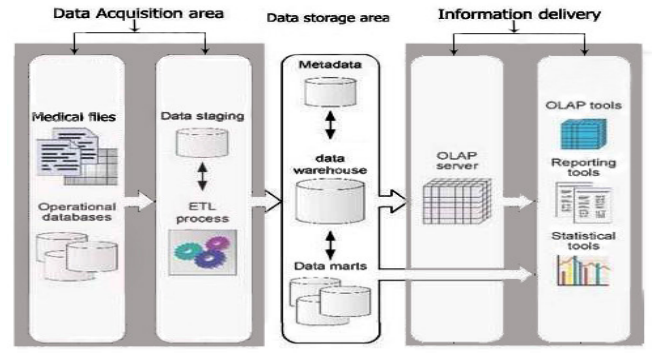
\includegraphics[width=0.75\textwidth]{images/chapter3/cancersystem.PNG}
      \caption{Cancer data warehouse Architecture Taken from the source.}
      \label{fig:cancersystem}
    \end{figure}
    \end{enumerate}
    
    \item \textbf{\textit{Data Warehouse Framework in Pharmaceutical Sector:}} In this paper\cite{abd2019proposed} authors proposed a data warehouse framework to enhance decisions of distribution systems in pharmaceutical companies to decrease the medicine industry cost and increase productivity. The framework can be described in four phases shown in (Figure \ref{fig:pharmacysystem}). Phase one consists of a data preparation, a phase which has four steps (data collection, building DBs, DWH and data cleaning). Phase two consists of training the data which is applying time series to three types of Neural Networks techniques (levenberg marquardt, Bayesian regularized, and Scaled conjugate gradient). Phase three is testing the performance based on mean square error (MSE). Phase four consists of evaluating the performance of the best prediction model.
    \begin{figure}[h!]
      \center
      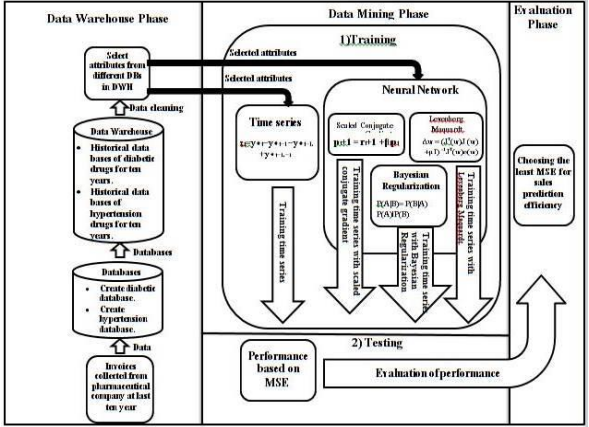
\includegraphics[width=0.75\textwidth]{images/chapter3/pharmacysystem.PNG}
      \caption{The Proposed Framework of Sales Prediction.}
      \label{fig:pharmacysystem}
    \end{figure}
    
    \item \textbf{\textit{Big Bata Warehouse Based On Hadoop Architecture:}} In this paper\cite{sebaa2018medical} entitled “Medical Big Data Warehouse: Architecture and System Design, a Case Study: Improving Healthcare Resources Distribution” authors proposed a system architecture and a conceptual data model for a MBDW (Medical Big Data Warehouse), and then offer a solution to overcome both the growing of fact table size and the lack of primary and foreign keys in the framework Apache Hive required in the conceptual data model. This solution is based on nested partitioning according to the dimension tables keys, then  applying their solution to implement a MBDW to improve medical resources distribution for the health sector in the Bejaia region (in Algeria). 
    \bigbreak
    The overall architecture is depicted in (Figure \ref{fig:bigdatarelated}). It is a scalable, reliable, and distributed architecture to extract, store, analyze, and visualize healthcare data extracted from various resources HIS (Hospitals Information systems).
    \begin{figure}[h!]
      \center
      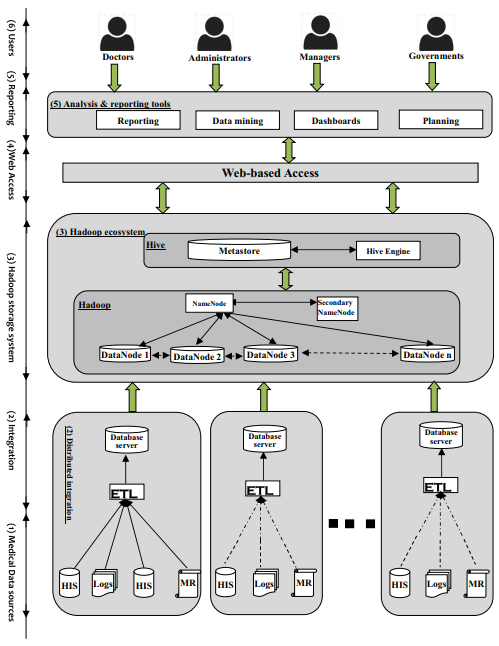
\includegraphics[width=0.50\textwidth]{images/chapter3/relatedworkHadoop.PNG}
      \caption{Hadoop-based system architecture of medical big data warehousing.}
      \label{fig:bigdatarelated}
    \end{figure}
\end{itemize}

\newpage
\section{Proposed Solution}
As mentioned in the project description, the presence of a visualization presentation in the medical sector is necessary. The proposed solution was to create a system that organizes the data and structures it, we used for that the eXtensible Markup Language (XML).
We mainly focused on the "Rendering" step in the visualization pipeline(\ref{fig:infovispipeline}), and we worked on the medical data that are mentioned in the Table\ref{tab:sourceTable}.

\subsection{Why XML?}
The rise of XML (eXtensible Markup Language) in patient care has been driven by the needs for communication among health professionals and between healthcare organizations such as hospitals and health insurance companies.The main advantage of XML is its flexibility, as it allows creators to describe any content easily by generating their own tags\cite{thuy2012s}. Some of XML’s features are\cite{achard2001xml}:
\begin{itemize}
\renewcommand{\labelitemi}{$\bullet$}
\item The XML and DTD files are human readable and thus can be easily edited by people with only a few computer skills. Updating a data model is, therefore, straightforward (at least from a technical point of view).
\item XML is Internet-oriented and has very rich capabilities for linking data; this can be used for interconnecting databases.
\item XML provides an open framework for defining standard specifications. This is an important point because medical informatics clearly lacks standardization. For example, querying on multiple molecular biology databases could be greatly facilitated if each database would offer an XML view of their content.
\end{itemize}
On the other hand, XML has some weaknesses:
\begin{itemize}
\renewcommand{\labelitemi}{$\bullet$}
\item The overhead of a text based format in data parsing, storage and transmission needs to be evaluated before adopting XML as a general solution. However, a text format means that the source code can be read and edited with any text editor.
\item It is not clear whether XML satisfactorily addresses the problems of technological scalability. Indeed if XML data are stored in flat files, queries on XML files will not scale because XML in itself does not provide scalable facilities such as indexing or data clustering. This means that parsing should be done on the fly which leads to poor performances. One solution could be to have query optimizations done externally for example using a DataBase Management System (DBMS).
\end{itemize}
\bigbreak
At this point the question to be answered is whether the pros prevail over the cons, for this reason Frederic Achard and al\cite{achard2001xml}  have provided a comparison between XML and some of the most popular solutions that are used for the management and exchange of bioinformatics data summarized in the (Table\ref{tab:xmlcomparaison}), each one is rated with one to four stars for different criteria: the higher the number of stars, the better the solution with regard to the criteria.
\begin{table}[h!]
    \centering
    \begin{tabular}{|m{0.20\linewidth}|m{0.10\linewidth}|m{0.10\linewidth}|m{0.10\linewidth}|m{0.11\linewidth}|m{0.10\linewidth}|m{0.10\linewidth}|}
        \hline

        \textbf{Criteria}                      & \textbf{XML}        & \textbf{{\small Field/ value} }        & \textbf{{\small \gls{asn}}}    & \textbf{{\small \gls{cobra}}} &\textbf{{\small \gls{java}}}      & \textbf{{\small \gls{oodbms}}}      \\

        \hline
        Model expressiveness 	& **	& *		& *** & *** & *** & ****     \\
        
        \hline
        Constraints	    & **	& *	& *    & **   & ***   & ****       \\
        
        \hline
        Self-descriptive    & yes	& no	& yes    & yes   &  yes  &  yes      \\
        
        \hline
        Query language	 & soon 	& no	& no    & soon    & no   &  yes \\
        
        \hline
        Flexibility	 & ****	& *	& ***    &  ***  & ***   & ****  \\
        
        \hline
        Simplicity 	 & ****	& ****	& ***    & *   & **   & **  \\
        
        \hline
        Scalability 	 & **	& *	& **   & ***   & ***   & ****  \\
        
        \hline
        Interoperability 	 & ****	& *	&  **  & ****   & ****   & ***  \\
                
        \hline
    \end{tabular} 

    \caption{Summary of comparison of different alternatives to XML.}
    \label{tab:xmlcomparaison}
\end{table}
\bigbreak
They conclude that the use of XML as an intermediate medium would be really efficient only if all databases share common or very similar DTDs. Whatever language is used, it is always difficult to find an agreement on a common semantics, and when one is found, it is often revised. However, XML would be an excellent candidate for this role because of its flexibility.



\subsection{Architecture}



We focused on extracting the following type of data (each head represents an XML node):
\begin{itemize}
\renewcommand{\labelitemi}{$\bullet$}
\item \textbf{Patient:} That presents the administrative information about the patient x, including his full name, gender, date of birth, address. 
\item \textbf{Drug:} Presents the list of drugs in the patient’s  prescription, it includes: the drug’s name, its dosage, strength usually mentioned by the doctor, the quantity, and its type(liquid or table).
\item \textbf{Diagnosis:} Includes the doctor's name, the diseases name, and the observations taken by the medical actor in charge, it also contains the name of the prescribed medications and the date of diagnosis. 
\item \textbf{LabResults:} It presents the medical biology results that includes the analysis’s name,the patient rate saved, the gender and the age for the comparison (a predefined high/low rate is defined corresponding to each analysis), attached with the laborator name.
\item \textbf{ImagesData:} Present the data of the image obtained by the patient, it includes the image name and the image itself, the day it was taken, and the patient's national ID number.
\end{itemize}
\begin{figure}[h!]
  \center
  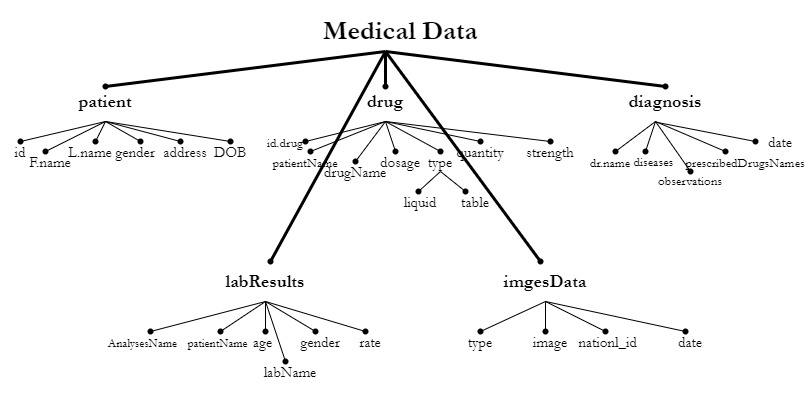
\includegraphics[width=0.99\textwidth]{images/chapter3/tree.jpg}
  \caption{The corresponding tree of XML schema.}
  \label{fig:xmlschema}
\end{figure}
\newpage
\subsection{Data Integration \& Processing}

Our main objective was to create a visualization system for that: we collected medical data from different sources that represent various medical actors, and we process them following the visualization process mentioned before (\ref{fig:infovispipeline}), we used Talend open studio (\ref{sec:talend}) to handle this step.

The resulting data will be used as a source to feed all the components of the digital marketing reporting applications that are built in many visualization tools.
\begin{figure}[h!]
  \center
  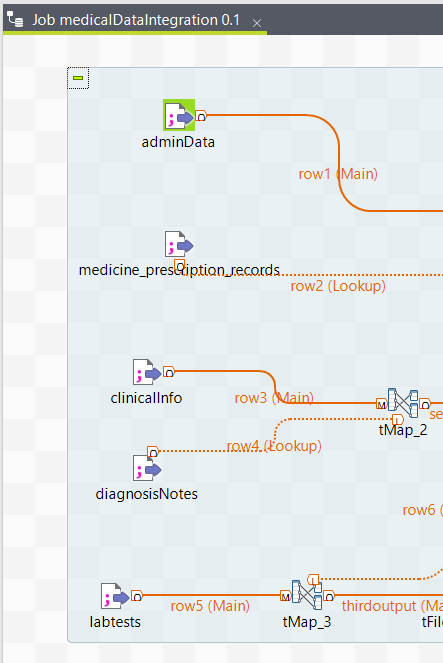
\includegraphics[width=0.30\textwidth]{images/chapter3/jobInputs.PNG}
  \caption{Input data.}
  \label{fig:jobinputes}
\end{figure}
\begin{figure}[h!]
  \center
  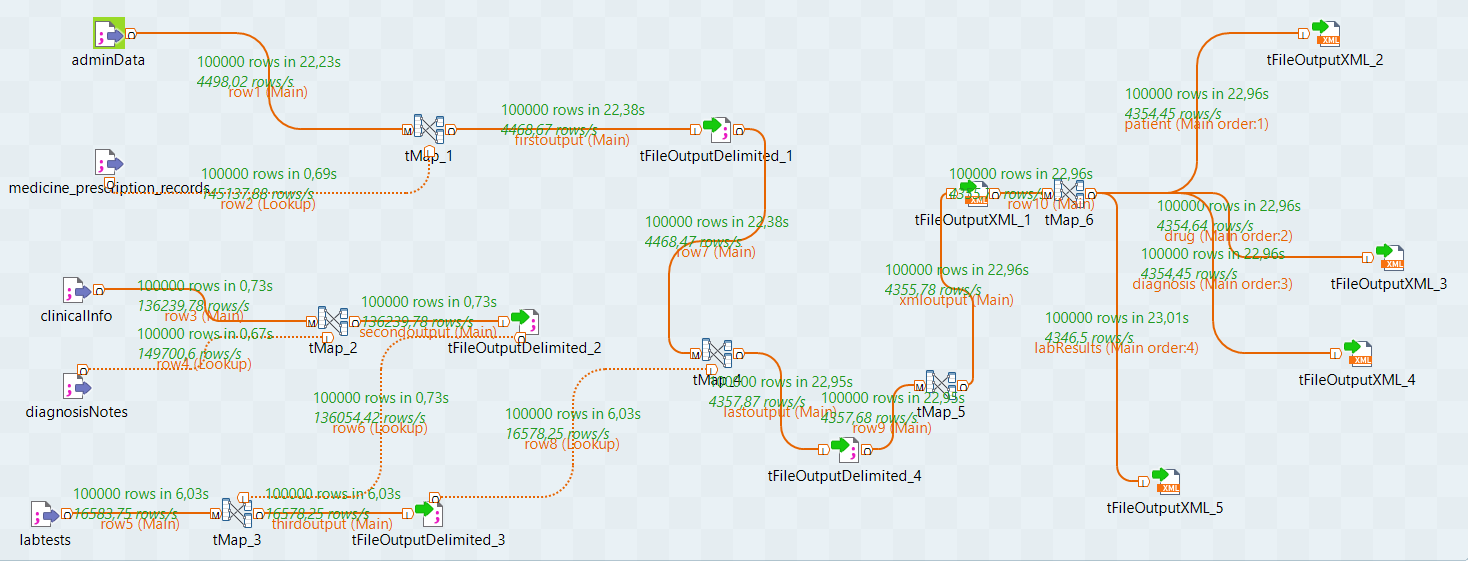
\includegraphics[width=0.80\textwidth]{images/chapter3/jobresult.PNG}
  \caption{Talend job execution.}
  \label{fig:jobtalend}
\end{figure}

\chapter{Implementation}
In this chapter, the process of implementation will be covered, starting by the architecture and the tools to the results and how everything fits together.

\section{Tools}
\subsection{Python}
Python\cite{WelcomePythonOrg} is a programming language that can be used in many contexts and is suitable for any type of use thanks to specialized libraries. However, it is particularly used as a scripting language to automate simple but tedious tasks. It is also used as a prototype development language when a functional application is needed before optimizing it with a lower level language. It is particularly widespread in the scientific world, and has many libraries optimized for numerical calculations\cite{PythonLangageWikipedia}.
\paragraph{Pandas:} 

Pandas\cite{PandasPythonData} is a library written for the Python programming language for data manipulation and analysis. In particular, it offers data structures and operations for manipulating numerical arrays and time series. Pandas is free software under the BSD license.


\begin{wrapfigure}[10]{r}{4cm}
	\vspace{-10pt}
	
\includegraphics[width=4cm]{images/chapter4/python_pandas.png}
	\vspace{-10pt}
	\caption{{\footnotesize Python et Pandas Logo.}}
\end{wrapfigure}


The main data structures offered by Pandas are series (to store data according to one dimension - size according to an index), DataFrames (to store data according to 2 dimensions - rows and columns), Panels (to represent data according to 3 dimensions, 4D Panels or Data Frames with hierarchical indexes also called Multi Index (to represent data according to more than 3 dimensions - hypercube))\cite{Pandas2020}.



\subsection{Talend}
\label{sec:talend}
We used  Talend Open Studio to create and develop ETL processes. It is a tool based on Java and with an interface derived from that of Eclipse (Figure \ref{fig:Talend}). It allows you to design ETL processes visually, and offers more than nine hundred components (the following list is not exhaustive)\cite{TalendOpenStudio}: 
\begin{itemize}
\item Connect to different data sources for reading and writing:
\begin{itemize}
\item Flat files, .xml, .csv, xls, etc.
\item Relational databases (Postgresql, MsSql, etc) and Nosql.
\end{itemize}
\item To manipulate the data, namely:
\begin{itemize}
\item Filter them.
\item Apply aggregate functions on them.
\item Sort them.
\end{itemize}
\item To organize data flows.
\end{itemize}
These components are then assembled as needed to design ETL processes\cite{mehdiPfe}.
\begin{figure}[h!]
    \center
    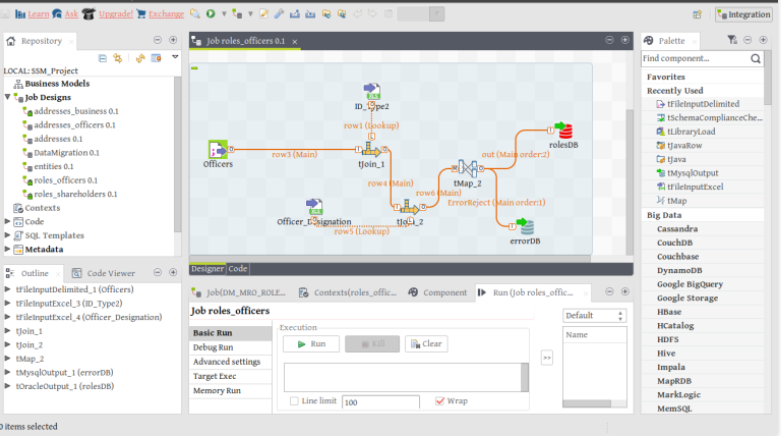
\includegraphics[width=0.75\textwidth]{images/chapter4/talendInterface.png}
    \caption{Talend Interface.}
    \label{fig:Talend}
\end{figure}
\newpage
\subsection{Tableau}
\label{sec:tableau}
Tableau is an excellent data visualization and business intelligence tool used for reporting and analyzing vast volumes of data. It helps users create different charts, graphs, maps, dashboards, and stories for visualizing and analyzing data, to help in making business decisions. Tableau supports powerful data discovery and exploration that enables users to answer important questions in seconds, it can connect to several data sources that other BI tools do not support. Tableau enables users to create reports by joining and blending different datasets and it supports a centralized location to manage all published data sources within an organization\cite{WhatTableauUltimate}.
\begin{figure}[h!]
    \center
    
\includegraphics[width=0.75\textwidth]{images/chapter4/TableauLogo.png}
    \caption{Tableau Logo.}
    \label{fig:tableau}
\end{figure}
\subsection{Highcharts}
Highcharts is a software library for charting written in pure JavaScript meant to enhance web applications by adding interactive charting capability. 
It has all the tools needed to create reliable and secure data visualizations by
providing a wide variety of charts. For example, line charts, spline charts, area charts, bar charts, pie charts and so on.They offer wrappers for the most popular programming languages (.Net, PHP, Python, R, Java) as well as iOS and Android, and frameworks like Angular, Vue, and React\cite{InteractiveJavascriptCharts}.
\begin{figure}[h!]
    \center
    
\includegraphics[width=0.25\textwidth]{images/chapter4/highchart.png}
    \caption{Highcharts Logo.}
    \label{fig:Highcharts}
\end{figure}

\section{Result}
To validate the proposed solution, we visualize the data  using various technologies highlighted in previous sections, in this section we will go through the results that were obtained by this investigatory effort.
\subsection{Processed Data Result}
After the data cleansing using python and its libraries, and the data processing using Talend, we got these results:


\begin{figure}[h!]
    \center
    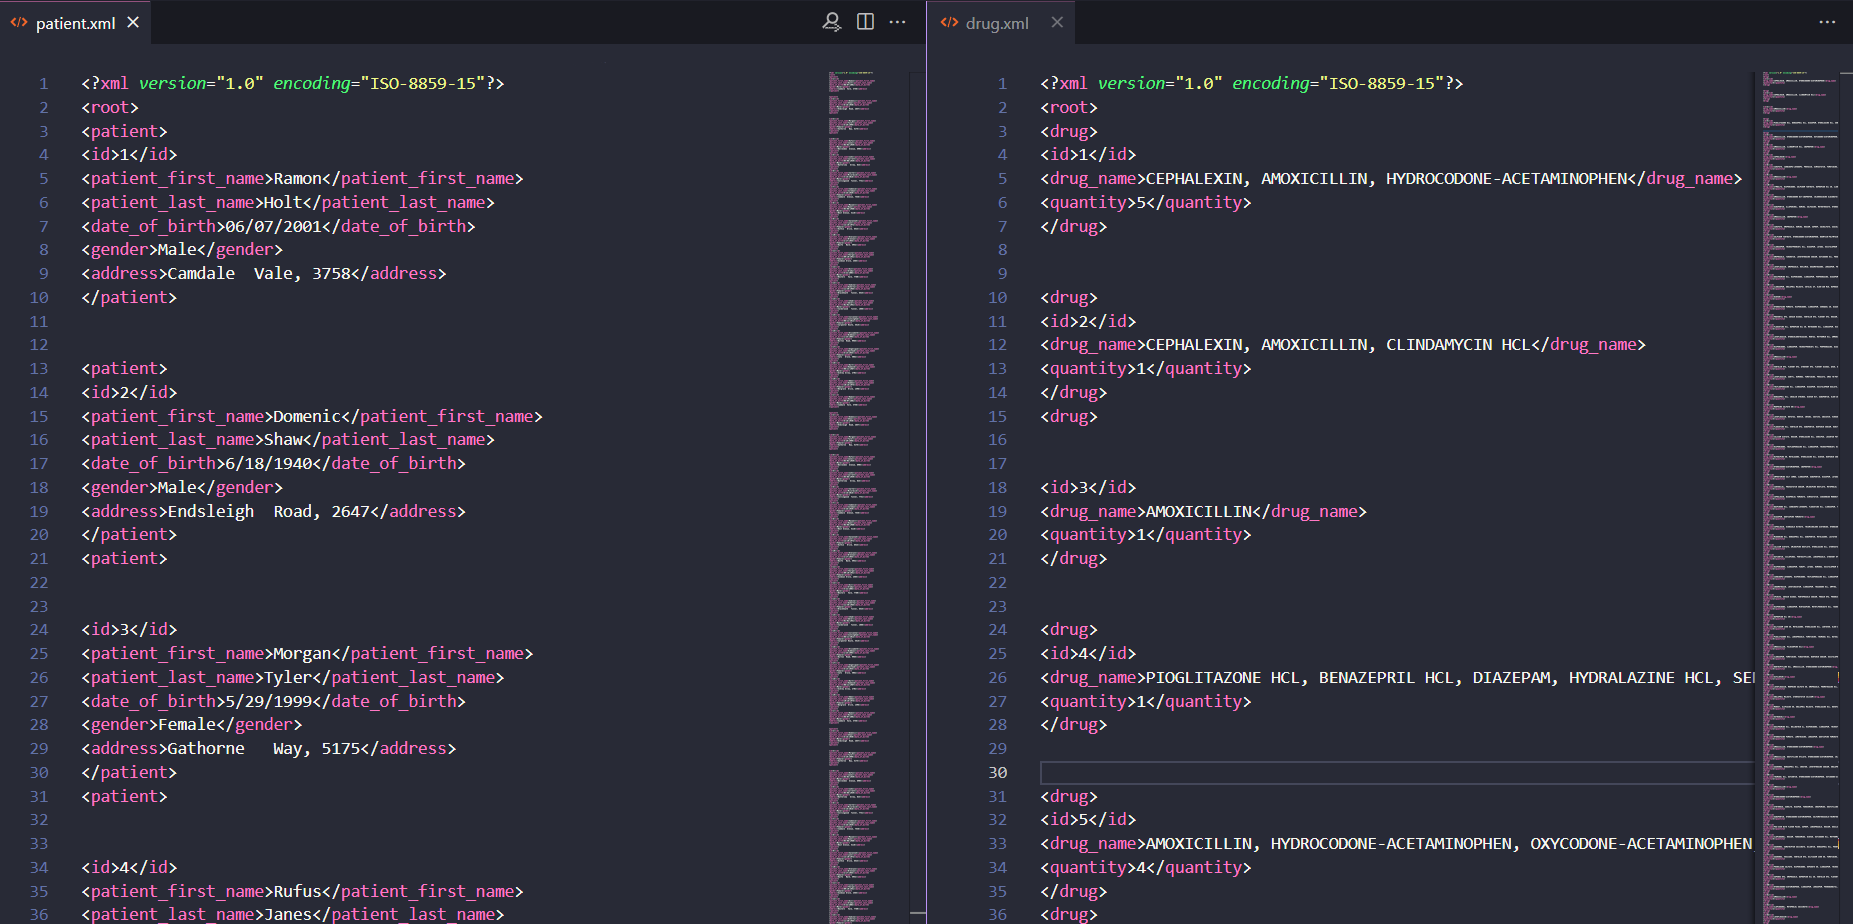
\includegraphics[width=0.90\textwidth]{images/chapter4/result1.PNG}
    \caption{Patient Informations and the related drugs.}
    \label{fig:resultone}
\end{figure}
\begin{figure}[h!]
    \center
    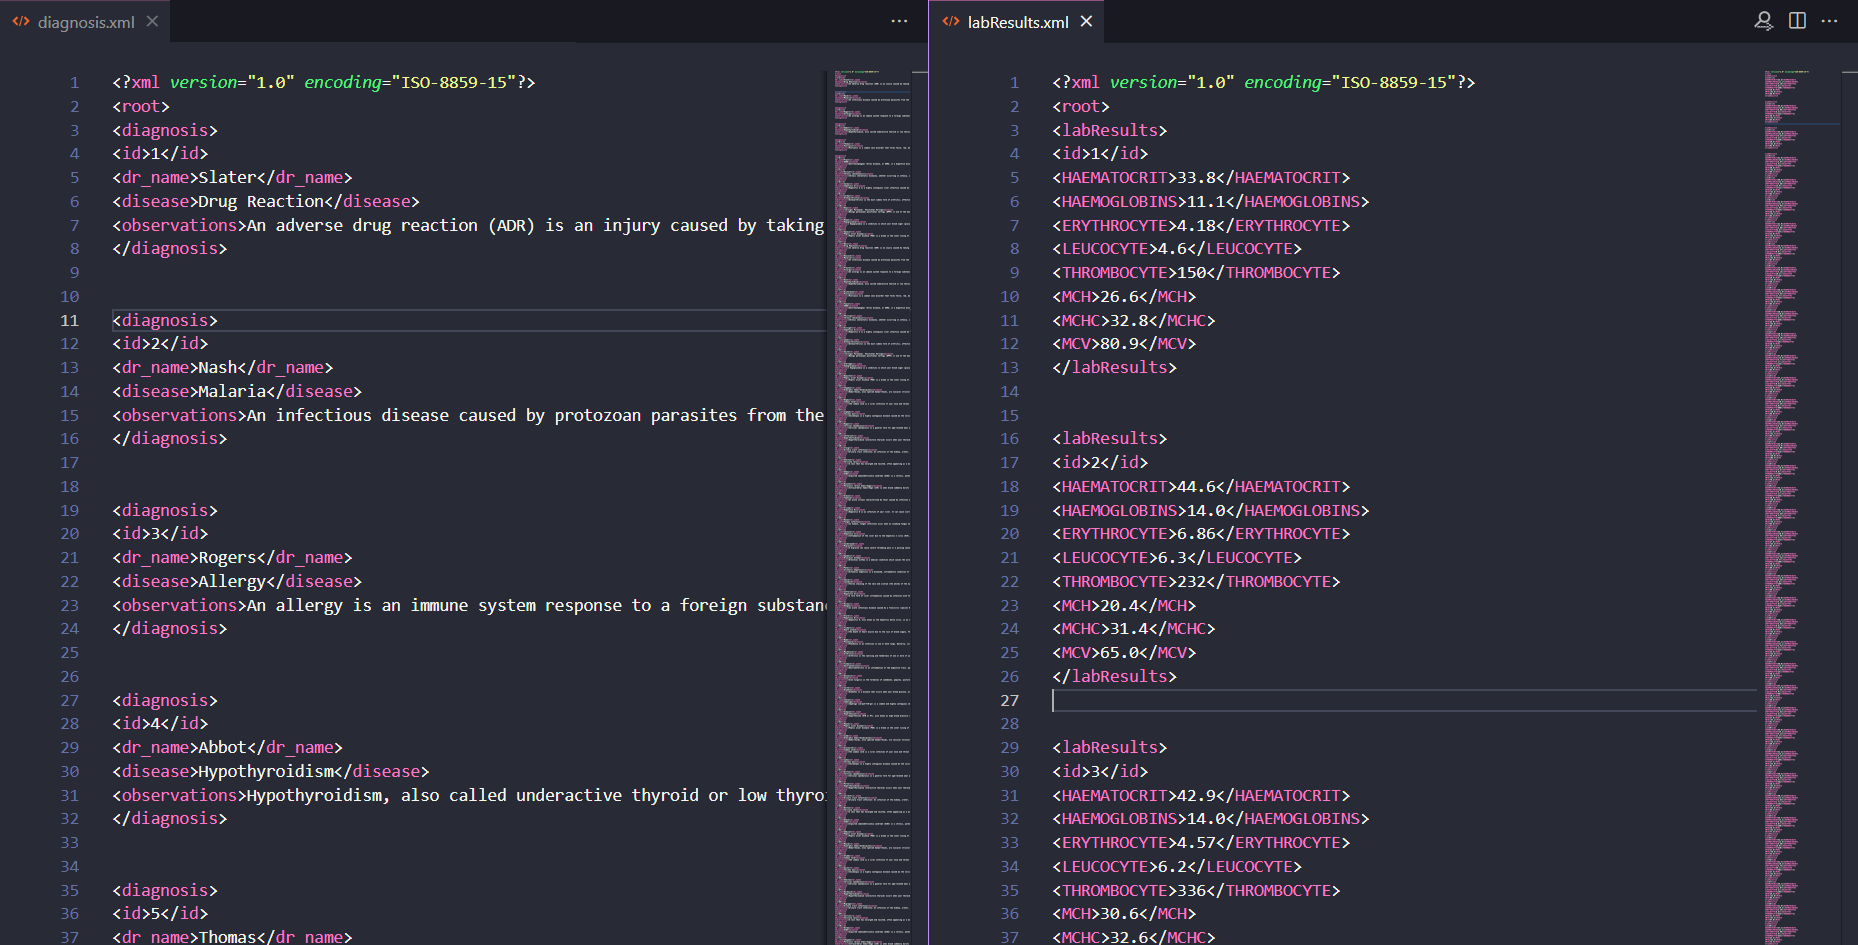
\includegraphics[width=0.90\textwidth]{images/chapter4/result2.PNG}
    \caption{Patient's diagnosis and the his Lab tests results.}
    \label{fig:resulttwo}
\end{figure}

\subsection{Dashboards}
The presented dashboards illustrate some different ways we can visualize some relevant patient data we obtained.\\
Both dashboards are a web application developed using bootstrap\cite{IntroductionBootstrapV5}  framework and the Highcharts  library.

\begin{itemize}
    \item \textbf{Administration Dashboard:}
     \begin{figure}[h!]
        \center
        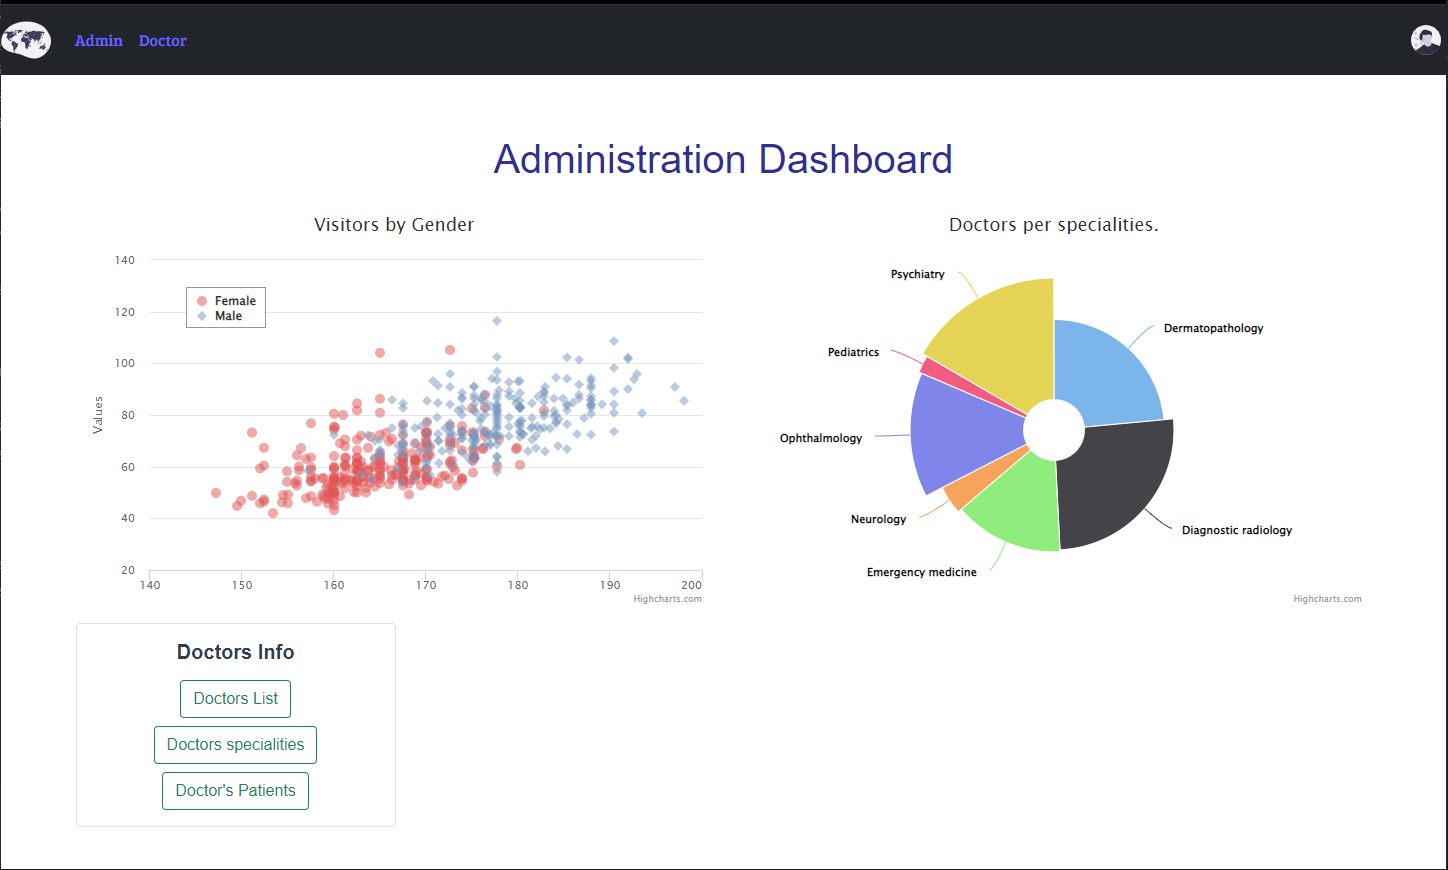
\includegraphics[width=0.90\textwidth]{images/chapter4/adminDashboard.PNG}
        \caption{Administration Dashboard illustrates some of Viz results.}
        \label{fig:admin}
    \end{figure}
    \newpage
    \item \textbf{Doctor Dashboard:}
    \begin{figure}[h!]
        \center
        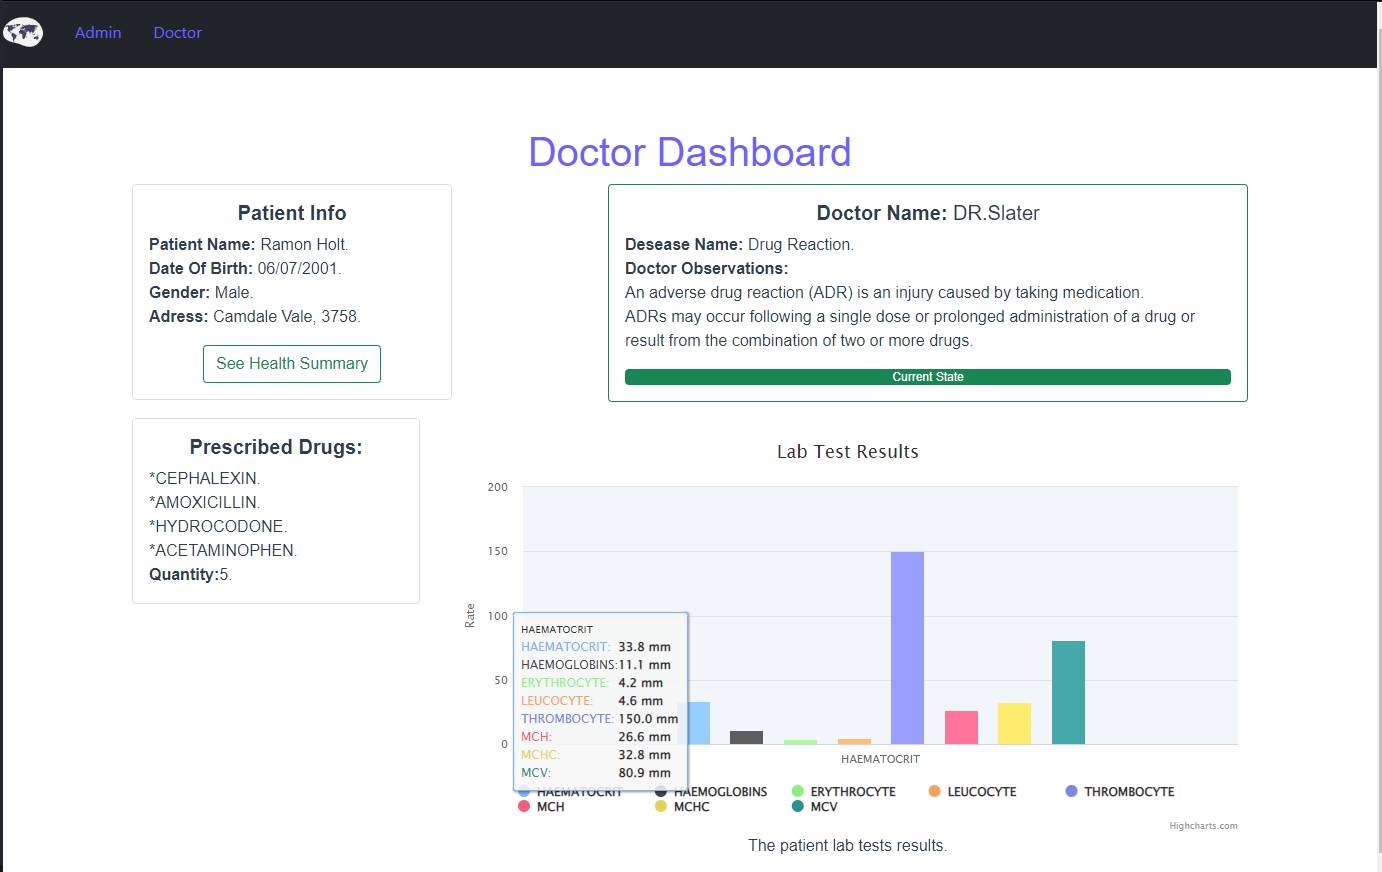
\includegraphics[width=0.90\textwidth]{images/chapter4/doctor.PNG}
        \caption{Doctor Dashboard.}
        \label{fig:doctor}
    \end{figure}
\end{itemize}
\chapter{Conclusion \& Future work}
During this graduation project, we touched on many areas in the world of medicine and informatics.Many technologies and tools have been explored over time, starting with data integration systems and analytics to visualization. Each technology represents a universe to be discovered and many others still remain to be explored in the field of data integration and analyses.
\bigbreak
In this thesis, we introduced medical informatics presenting all the data types and actors contributing to it. We also presented the visualization field and the visualization pipeline and we have seen the data warehouse definition and the various data integration approaches.
In our work, we presented a visualization system that deals with multiple data sources and produces a structured data form presented in an XML form that could be easily visualized to the multiple medical actors. However, it will be necessary to ensure to have the right tools and good practices. In our case, we were limited to open source tools and hardware, which severely limited us.
\bigbreak
This work remains a first version made using the relatively limited means at our disposal. But it remains a good starting point that would be interesting to develop. Several points could improve this system, we mention:
\begin{itemize}
\item Introduce continuous data integration.
\item Mixe the processing step by machine learning systems.
\item Get the system protected using some security systems.
\item Offer different outputs depending on what the actor needs.
\end{itemize}

\bibliographystyle{plain}
\bibliography{biblo.bib}
\end{document}
